\begin{figure}[htb!]
  \centering
  \begin{subfigure}[b]{0.25\textwidth}
    \centering
    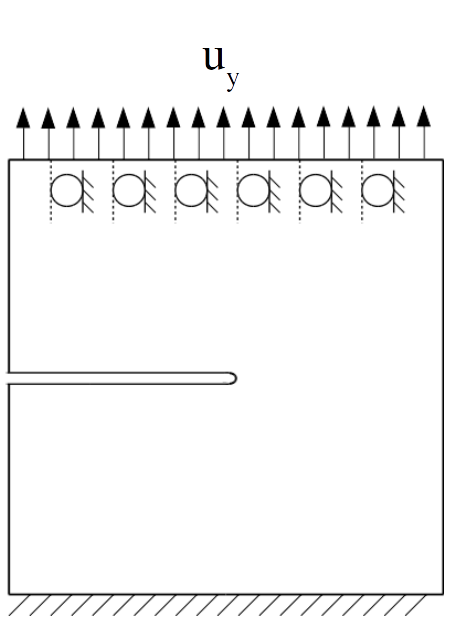
\includegraphics[width=0.8\textwidth,scale=0.5]{Chapter4/figures/mode1_bcs}
    \caption{}
    \label{fig: Chapter4/mode1_bcs}
  \end{subfigure}
  \hspace{0.03\textwidth}
  \begin{subfigure}[b]{0.19\textwidth}
    \centering
    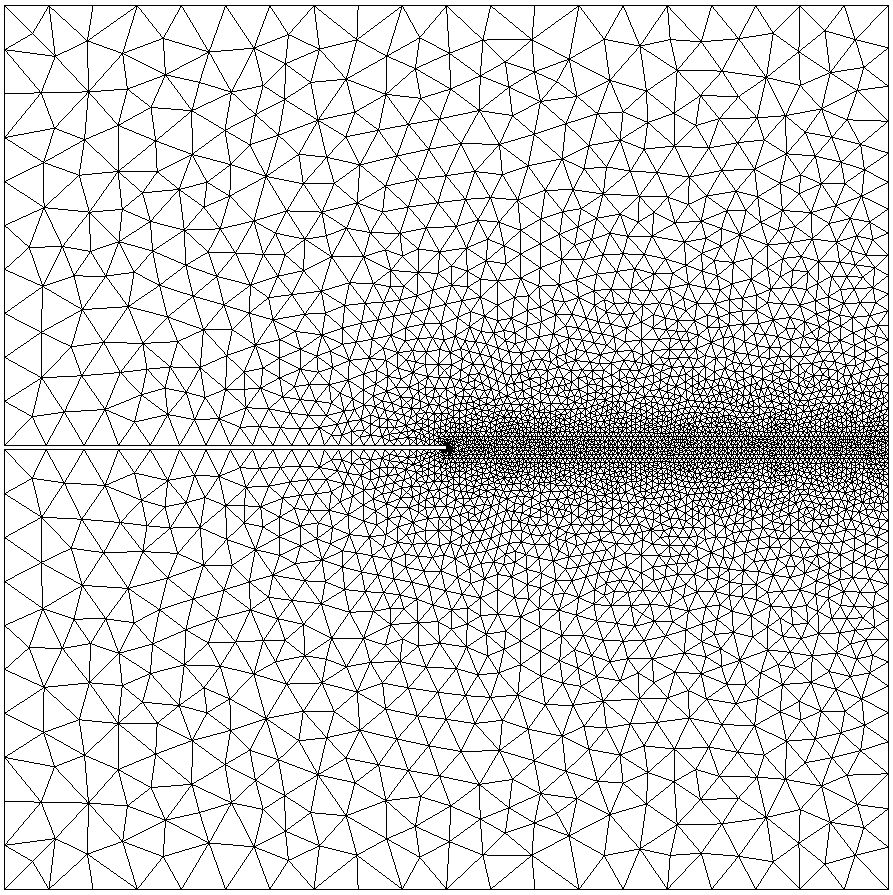
\includegraphics[width=\textwidth]{Chapter4/figures/mode1_notch_mesh.png}
    \caption{}
    \label{fig: Chapter4/mode1_notch_mesh}
  \end{subfigure}
  \hspace{0.05\textwidth}
  \begin{subfigure}[b]{0.19\textwidth}
    \centering
    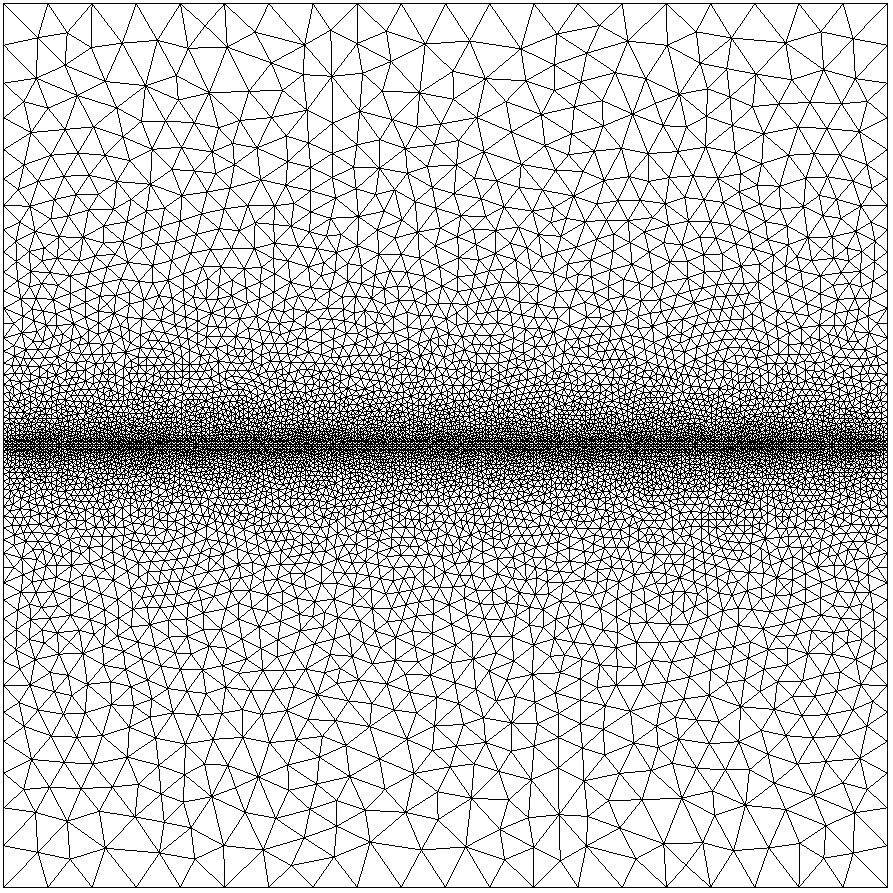
\includegraphics[width=\textwidth]{Chapter4/figures/mode1_initial_mesh.png}
    \caption{}
    \label{fig: Chapter4/mode1_initial_mesh}
  \end{subfigure}
  
  \begin{subfigure}[b]{0.25\textwidth}
    \centering
    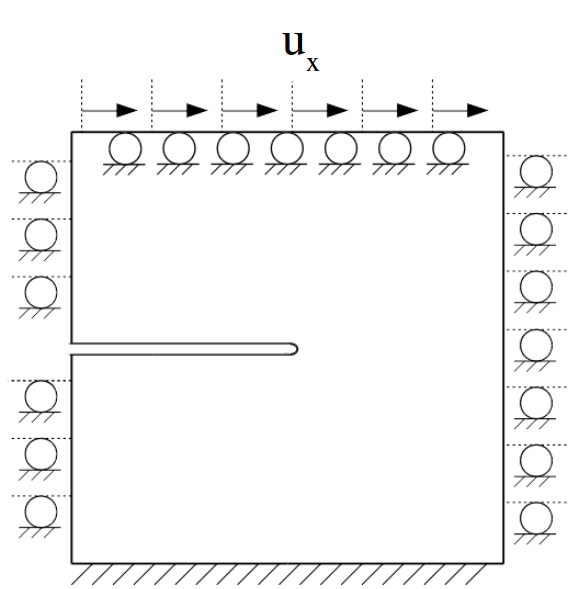
\includegraphics[width=\textwidth,scale=0.5]{Chapter4/figures/mode2_bcs.png}
    \caption{}
    \label{fig: Chapter4/mode2_bcs}
  \end{subfigure}
  \hspace{0.03\textwidth}
  \begin{subfigure}[b]{0.19\textwidth}
    \centering
    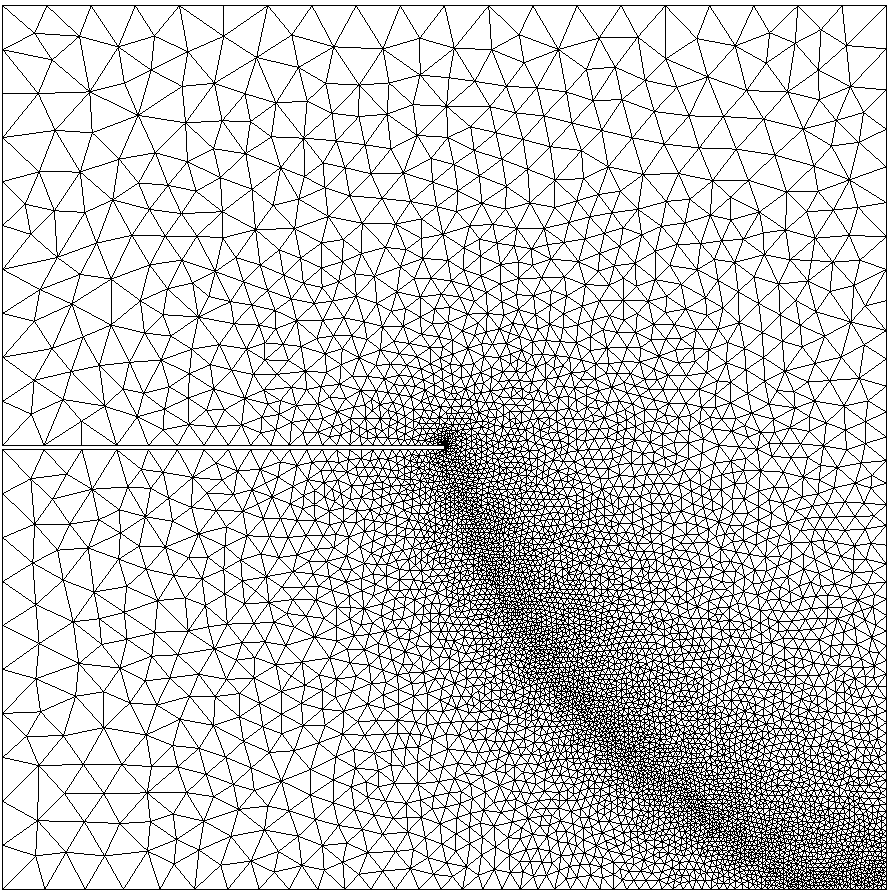
\includegraphics[width=\textwidth]{Chapter4/figures/mode2_notch_mesh.png}
    \caption{}
    \label{fig: Chapter4/mode2_notch_mesh}
  \end{subfigure}
  \hspace{0.05\textwidth}
  \begin{subfigure}[b]{0.19\textwidth}
    \centering
    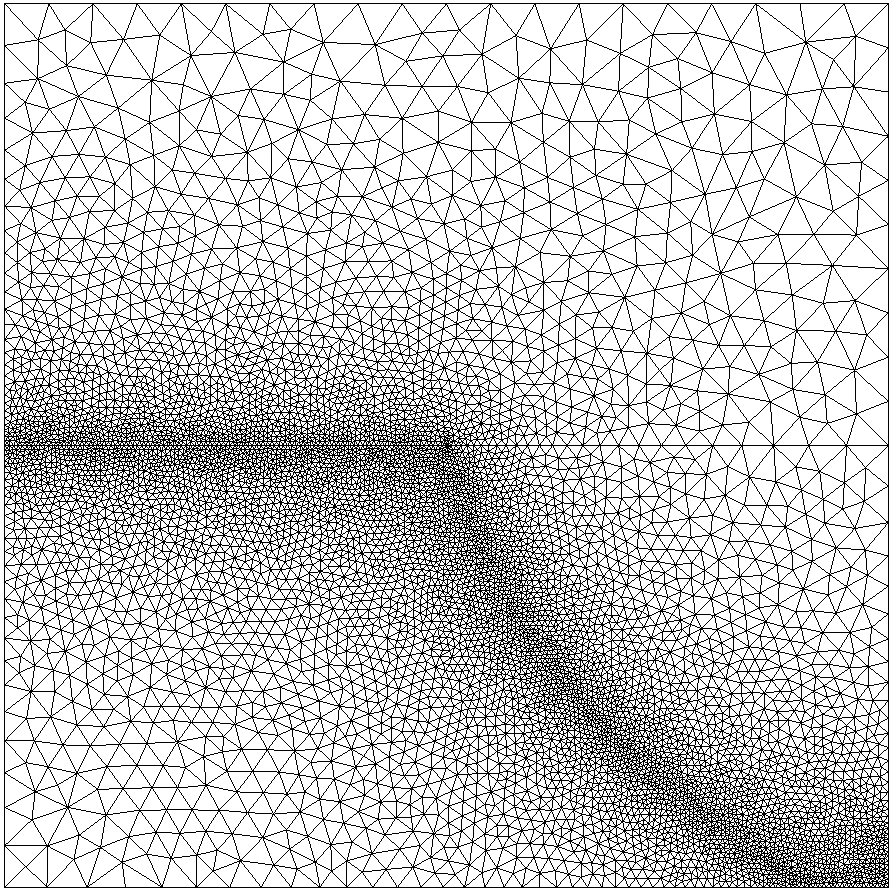
\includegraphics[width=\textwidth]{Chapter4/figures/mode2_initial_mesh.png}
    \caption{}
    \label{fig: Chapter4/mode2_initial_mesh}
  \end{subfigure}
  \caption[Boundary conditions of the plate with a pre-existing crack for a mode I tension test and a mode II shear test.]{Boundary conditions of the plate with a pre-existing crack for (a) a mode I tension test and (d) a mode II shear test. Finite element meshes for the mode I calculations (b - c) and for the mode II calculations (e - f). For (b, e) the meshes have the initial crack geometry ``meshed-in'' while (c, f) have local refinement around the initial phase field. All meshes are pre-refined along the predicted crack-path with a characteristic element size of \SI{0.005}{\milli\meter}.}
  \label{fig: example/bcs}
\end{figure}
